

\section{Results}

\subsection{Position dependence}

Figure \ref{fig:pos_dependence_aes} shows the position dependence of the AES2 signal. Figure \ref{fig:pos_dependence_aes}A shows the AES2 absorption spectra for a range of positions along the free jet, along with fits. 

Figure \ref{fig:pos_dependence_aes} B and C show the potassium number density obtained from the $\alpha$ fit for different positions along the torch axis, and 0.8 and 0.6 equivalence ratio. The potassium measurement at the barrel exit throughout the position sweep is also shown. The CFD data is sampled along a line on the torch axis, either directly on the torch axis or offset perpendicular to simulate misalignment in the AES2 beam. 

\begin{figure}[h]
    
\includegraphics[width=0.8\linewidth]{\repodir/final/figures/output/Fig3_Position_AES.png} 
    \caption{AES Measurements: A) AES absorption spectra and fits for a few positions along the free jet. B) Position dependence of atomic potassium as measured by AES and predicted by CFD for 1 \% seed and an equivalence ratio of 0.8. The CFD data is sampled along a line on the torch axis, either directly on the torch axis or offset perpendicular to simulate misalignment in the AES beam. C) The same as B, but for an equivalence ratio of 0.59. }
    \label{fig:pos_dependence_aes}
\end{figure}

Figure \ref{fig:pos_dependence_mws} examines the position dependence of the MWS signal at a fixed 1 \% potassium mass fraction (536\_pos).  These measurements are used to motivate the nominal stage position of 180 mm downstream of the jet which is used for the fixed position Kwt dependence (53x) measurements presented in the next section. 

Figure \Ref{fig:pos_dependence_mws}A and B show the $\Delta AS$ signal at a position of 105 mm and 180 mm downstream of the barrel exit, respectively. In \ref{fig:pos_dependence_mws}A individual test case profiles are shown. We observe that near the exit of the torch (including 105 mm position) there is a significant fluctuation in the MWS signal in the absence of a laser pulse. These fluctuations can be observed in the $\Delta AS$ signal, where the underlying transmission magnitude is fluctuating and causing the $\Delta AS$ signal to above and below the zero line. As mentioned previously, the $\Delta AS$ signal is calculated with respect to a time window of 1 $\mu s$ before the laser pulse, and therefore deviations in transmission magnitude prior to the laser pulse can cause the $\Delta AS$ signal to fluctuate below zero.

For the present discussion, the important point is that these fluctuations are significant compared to the signal induced by the laser pulse, and they therefore preclude accurate measurement of the time decay of the AS signal after the laser pulse. The source of these fluctuations is not investigated in detail in the present work, but presumably the temperature at the exit of the torch is sufficiently high for thermally induced conductivity. Variations in the flow or potassium distribution could cause these time dependent fluctuations. 

In Figure \ref{fig:pos_dependence_mws}B the $\Delta AS$ signal is shown at 180 mm downstream of the barrel exit. The background fluctuations in the $\Delta AS$ signal are significantly reduced compared to the 105 mm position, but a significant $\Delta AS$ response from the laser is still observed. 

In Figure \ref{fig:pos_dependence_mws}C we show the maximum of the $\Delta AS$ signal within 1 $\mu s$ of the laser pulse (0 $\mu s$) as a function of stage position, $\Delta AS_{max}$. The maximum of the $\Delta AS$ signal is used as a measure of the signal strength. The maximum of the $\Delta AS$ signal is observed to increase with stage position, and then decrease.


To determine the nominal location for measurement of the potassium dependence, we define a signal to fluctuation ratio (SFR): 

\begin{equation}
    \label{eq:sfr}
    SFR = \frac{\Delta AS_{max}}{U_{std,PP}}
\end{equation}

Where $U_{std,PP}$ is the standard deviation of the MWS magnitude in the time window of -50 to -1 $\mu s$ before the laser pulse.  In figure \ref{fig:pos_dependence_mws}D we examine the SFR as a function of stage position to find the optimal position for the MWS diagnostic. We observe that similar to $\Delta AS_{max}$, $U_{std,PP}$ increases downstream of the torch, and decreases (SI). However, $PP_{std}$ decreases more rapidly than $AS_{max}$, so the signal to fluctuation ratio increases to a maximum at approximately 180 mm downstream from the torch. 


\begin{figure}[h]
    
\includegraphics[width=0.8\linewidth]{\repodir/final/figures/output/Fig4_Position_MWS.png} 
    \centering
    \caption{Position dependence of the MWS signal. The data are taken for full laser power and 1\% nominal K mass fraction. All error bars are standard deviation across Runs.  A) AS profiles taken at 105 mm downstream of the barrel exit The hue represents different repeats of the test case sequence, with each line being an average of all oscilloscope acquisitions in a given test case.  B) The AS signal further downstream at the nominal position of 180 mm. The confidence interval represents the standard deviation across runs C)  The maximum of the $\Delta AS$ signal within 1 $\mu s$ of the laser pulse (0 $\mu s$).  D) The ratio of the Max AS and pre-pulse magnitude standard deviation, a measure of the signal to noise ratio. For C, and D the error bars represent the standard deviation across runs. Vertical dashed lines represent the positions shown in A and B. Note that on 2023-05-12, position dependent measurements were performed on a different but semi-overlapping set of positions (including the nominal position), leading to the datapoints with zero error bars. } 
    \label{fig:pos_dependence_mws}
\end{figure}


Together the position (Figure \ref{fig:pos_dependence_mws}) and the power dependence (Figure S\ref*{fig:SI_power_dependence}) motivate the conditions used for the Kwt dependence presented below: Measurements are taken at 180 mm downstream of the barrel in order to maximize the signal to fluctuation ratio and accurately measure the profile of the AS decay after the laser pulse. We note, as discussed further later, that the AS decay rate does not appear to depend sensitively on the position (see \ref{fig:pos_dependence_mws} and SI). We take measurements at full laser power (~7 mJ) to maximize the signal and as the exponential time constant does not appear to depend sensitively on the laser power (SI).

\clearpage

\subsection{Potassium dependence}

Figure \ref{fig:kwt_ionization} shows results with the mobile setup positioned at 180 mm and full laser power, while varying the nominal potassium mass fraction. Figure \ref{fig:kwt_ionization}A shows the potassium number density, $n_K$, as measured by both AES diagnostics, compared to species densities predicted by CFD. The barrel measurement of the $n_K$ is observed to increase with the nominal potassium mass fraction, as expected. However, $n_K$ at the goldilocks position has a slight decrease as a function of increasing nominal mass fraction. The CFD predictions for K, KOH, and all K species are also shown. The CFD results are consistent with the measurements. The CFD K density at the goldilocks position is similar to the experimental results, and the K species sum at the goldilocks position is consistent with the AES2 measurements at the barrel. Additionally, nearly all K species are predicted to predicted to be in the form of KOH at the goldilocks position. Together, these results suggest that the temperature of the jet has reduced sufficiently that the potassium is primarily in the form of KOH at the goldilocks position.

Figure  \ref{fig:kwt_ionization}B shows $\Delta AS$ as well the on-peak PD signal as a function of nominal potassium mass fraction. The photodiode signal is from the on-peak (K filtered) photodiode and is the difference between the maximum of the signal in time and the signal 1 $\mu s$ before the laser pulse. Both signals are observed to increase with the nominal potassium mass fraction. 

\begin{figure}[h]
    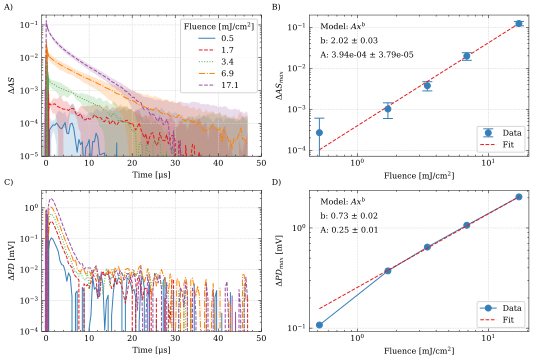
\includegraphics[width=0.8\linewidth]{\repodir/final/figures/output/Fig5_Kwt_Ionization.png} 
    \caption{Kwt dependence of Ionization related parameters. Measurements and predictions are for the free jet at the nominal position of 180 mm or exit of the HVOF barrel. measurements are for full laser power as a function of nominal potassium weight percent at 0.8 equivalence ratio. A) species number density results and CFD predictions. Goldi = Goldilocks. B) MWS AS maximum (within 1 us of laser pulse) and photodiode signal. The photodiode signal is from the on-peak (K filtered) photodiode and is the difference between the maximum of the signal in time and the signal 1 us before the laser pulse.  }
    \label{fig:kwt_ionization}
\end{figure}


Figure \ref{fig:kwt_recombination} shows analysis of the $\Delta AS$ decay measurements as a function of nominal potassium mass fraciton.  Figure \ref{fig:kwt_recombination}A shows the $\Delta AS$ time profile for a range of K mass fraction. Immediately after the laser pulse, there is a region of of changing slope in the logarithm of the $\Delta AS (t)$ profile. After a few microseconds, the profile becomes an exponential decay. Assuming, $\Delta AS (t) \propto \Delta n_e (t)$, where $\Delta n_e (t)$ is the time dependent change in the free electron density from the steady state concentration, we derive in the SI a differential equation for the decay of $\Delta n_e (t)$. In the regime where $\Delta n_e (t)$ is small, the equation has the exponential form.  

\begin{equation}
    \label{eq:fit_eq}
    \frac{d\Delta n_e (t)}{dt} = - k_{r, m, eff} \Delta n_e (t) 
\end{equation}

The time constant of the exponential decay for capture with species X, $\tau$, is given by

\begin{equation}
    \label{eq:tau_krm}
    k_{r, m, X} = \frac{1}{\tau} = k_{r, b, X}n_{X,0}
\end{equation}

Where, $\tau$ is the exponential time constant and $n_{X,0}$ is the equilibrium species concentration of X, and $k_{r, b, X}$ is the bimolecular recombination rate coefficient for capture by X. The fitted time constants are shown in Figure \ref{fig:kwt_recombination}B.


\begin{figure}[h]
    
\includegraphics[width=0.8\linewidth]{\repodir/final/figures/output/Fig6_Kwt_Recombination.png} 
    \centering
    \caption{Kwt dependence of the MWS decay. A) MWS $\Delta AS$ time profiles for different potassium mass fractions. The black lines are exponential fits. B) Decay time constants associated with equation \ref{eq:tau_krm}. The time constant is measured experimentally through and exponential fit of the AS signal. The CFD predictions are based on the literature rate cosntants and CFD species number densities at the goldilocks position as discussed in the text.  }
    \label{fig:kwt_recombination}
\end{figure}



We calculate expected decay constants for electron capture by various species in \ref{fig:kwt_recombination}B to compare to the experimental decay constant. The expected decay constants are calculated through equation \ref{eq:tau_krm} with $n_{X,0}$ given by the CFD results at the goldilocks position. For $k_{r,b,X}$, we have searched for data on reaction kinetics that are compatible with first-order recombination of electrons (eq. \ref{eq:fit_eq}) which are summarized in Table \ref{tab:reactions}. For some reactions and $k_{r,b,X}$ is given directly in the literature in units of $cm^3/s$. Some reactions are termolecular and further depend on a collisional partner, M, and are of the form [X] +[e-] + M \rightarrow [X-] + M. in this case $k_{r,b} = k_{r,tm} [M]$, where $k_{r,tm}$ is the termolecular recombination rate given in units of $cm^6/s$ and [M] is the number density of the collision partner.  The densities of [M] and [X] are taken from the CFD results at the goldilocks position. For the OH and K capture reactions, we use the number density of the entire flame as the collisional partner. 


\begin{table}[h]
\centering
\caption{Collected Reaction Kinetics for Electron Recombination.}
\label{tab:reactions}
\begin{tabular}{|c|c|c|c|}
\hline
Name & Reaction & Rate Coefficient & Reference \\
\hline
K$^+$ & K$^+$ + e$^-$ + M $\rightarrow$ K + M & $4 \times 10^{-24}$ T$^{-1}$ cm$^3$/s & Jensen 1978 \\
\hline
O2\_A & O$_2$ + e$^-$ + M $\rightarrow$ O$_2^-$ + M & $5 \times 10^{-31} cm^6/s$ & Axford 1997 \\
\hline
O2\_B & ""                                          & $6 \times 10^{-34} cm^6/s$ &  Goodings 1979 \\
\hline
O2\_C & ""                                          & Weighted sum  &  Axford 1997 \\
\hline
OH & OH + e$^-$ + M $\rightarrow$ OH$^-$ + M & $3 \times 10^{-31}$ cm$^6$/s & Axford 1997 \\
\hline
H$_2$O & H$_2$O + e$^-$ $\rightarrow$ H$_2$O$^-$ & $1.6 \times 10^{-6}$ exp(36060/T) cm$^3$/s & Axford 1997 \\
\hline
\end{tabular}
\end{table}

For recombination with molecular oxygen, there is significant uncertainty in the rate constant and we consider a few possibilities indicated in the legend of \ref{fig:kwt_recombination}C. Axford 1997 discussed this uncertainty and presented a range of rate constants ultimately deciding on a value of $5e-31 cm^6/s$ for their H2 + O2 + N2 flame, which we consider as '$O2_A$' using the number density of all species as the collisional partner density. In the same discussion they specify the dominant collisional partners of the various literature values of the rate constant, so for '$O2_C$' we preform a sum of species dependent $k_{r,tm}$ with the CFD number densities for each collisional partner to determine an overall $k_r$. The constants presented by Axford 1997 include low temperature measurements, but mention that $k_{r,th}$ is expected to decrease at flame temperatures. Goodings 1979 found a much lower rate constant for similar flames and speculated a large negative temperature coefficient for the oxygen capture reaction. We consider this as '$O2_B$' and use the number density of all species as the collisional partner density. It is not clear why Axford 1997 did not mention the Goodings 1979 result (Hayhurst was on both papers). 

In summary there is a large uncertainty in the $k_{r,th}$ for the oxygen capture reaction. We present a range of predictions in \ref{fig:kwt_recombination}C. Our results fall within this large deviation. All other reactions predict decays much longer than the observed experimental decay. 

We note that the previously mentioned sources have much better agreement on the OH, H2O, and K capture reactions than the O2 capture reactions. 



